\documentclass[tikz,border=0pt]{standalone}
\usepackage[american]{circuitikz}
\usetikzlibrary{arrows.meta,calc,positioning,decorations.pathmorphing,patterns}
\definecolor{zyloTeal}{HTML}{174A5B}
\definecolor{zyloTealTwo}{HTML}{246B7A}
\definecolor{zyloInk}{HTML}{1F2933}
\definecolor{zyloSoft}{HTML}{EAF4F4}
\definecolor{zyloPaper}{HTML}{F8FAFB}
\definecolor{zyloLine}{HTML}{44606B}
\definecolor{zyloOrange}{HTML}{D97706}
\begin{document}
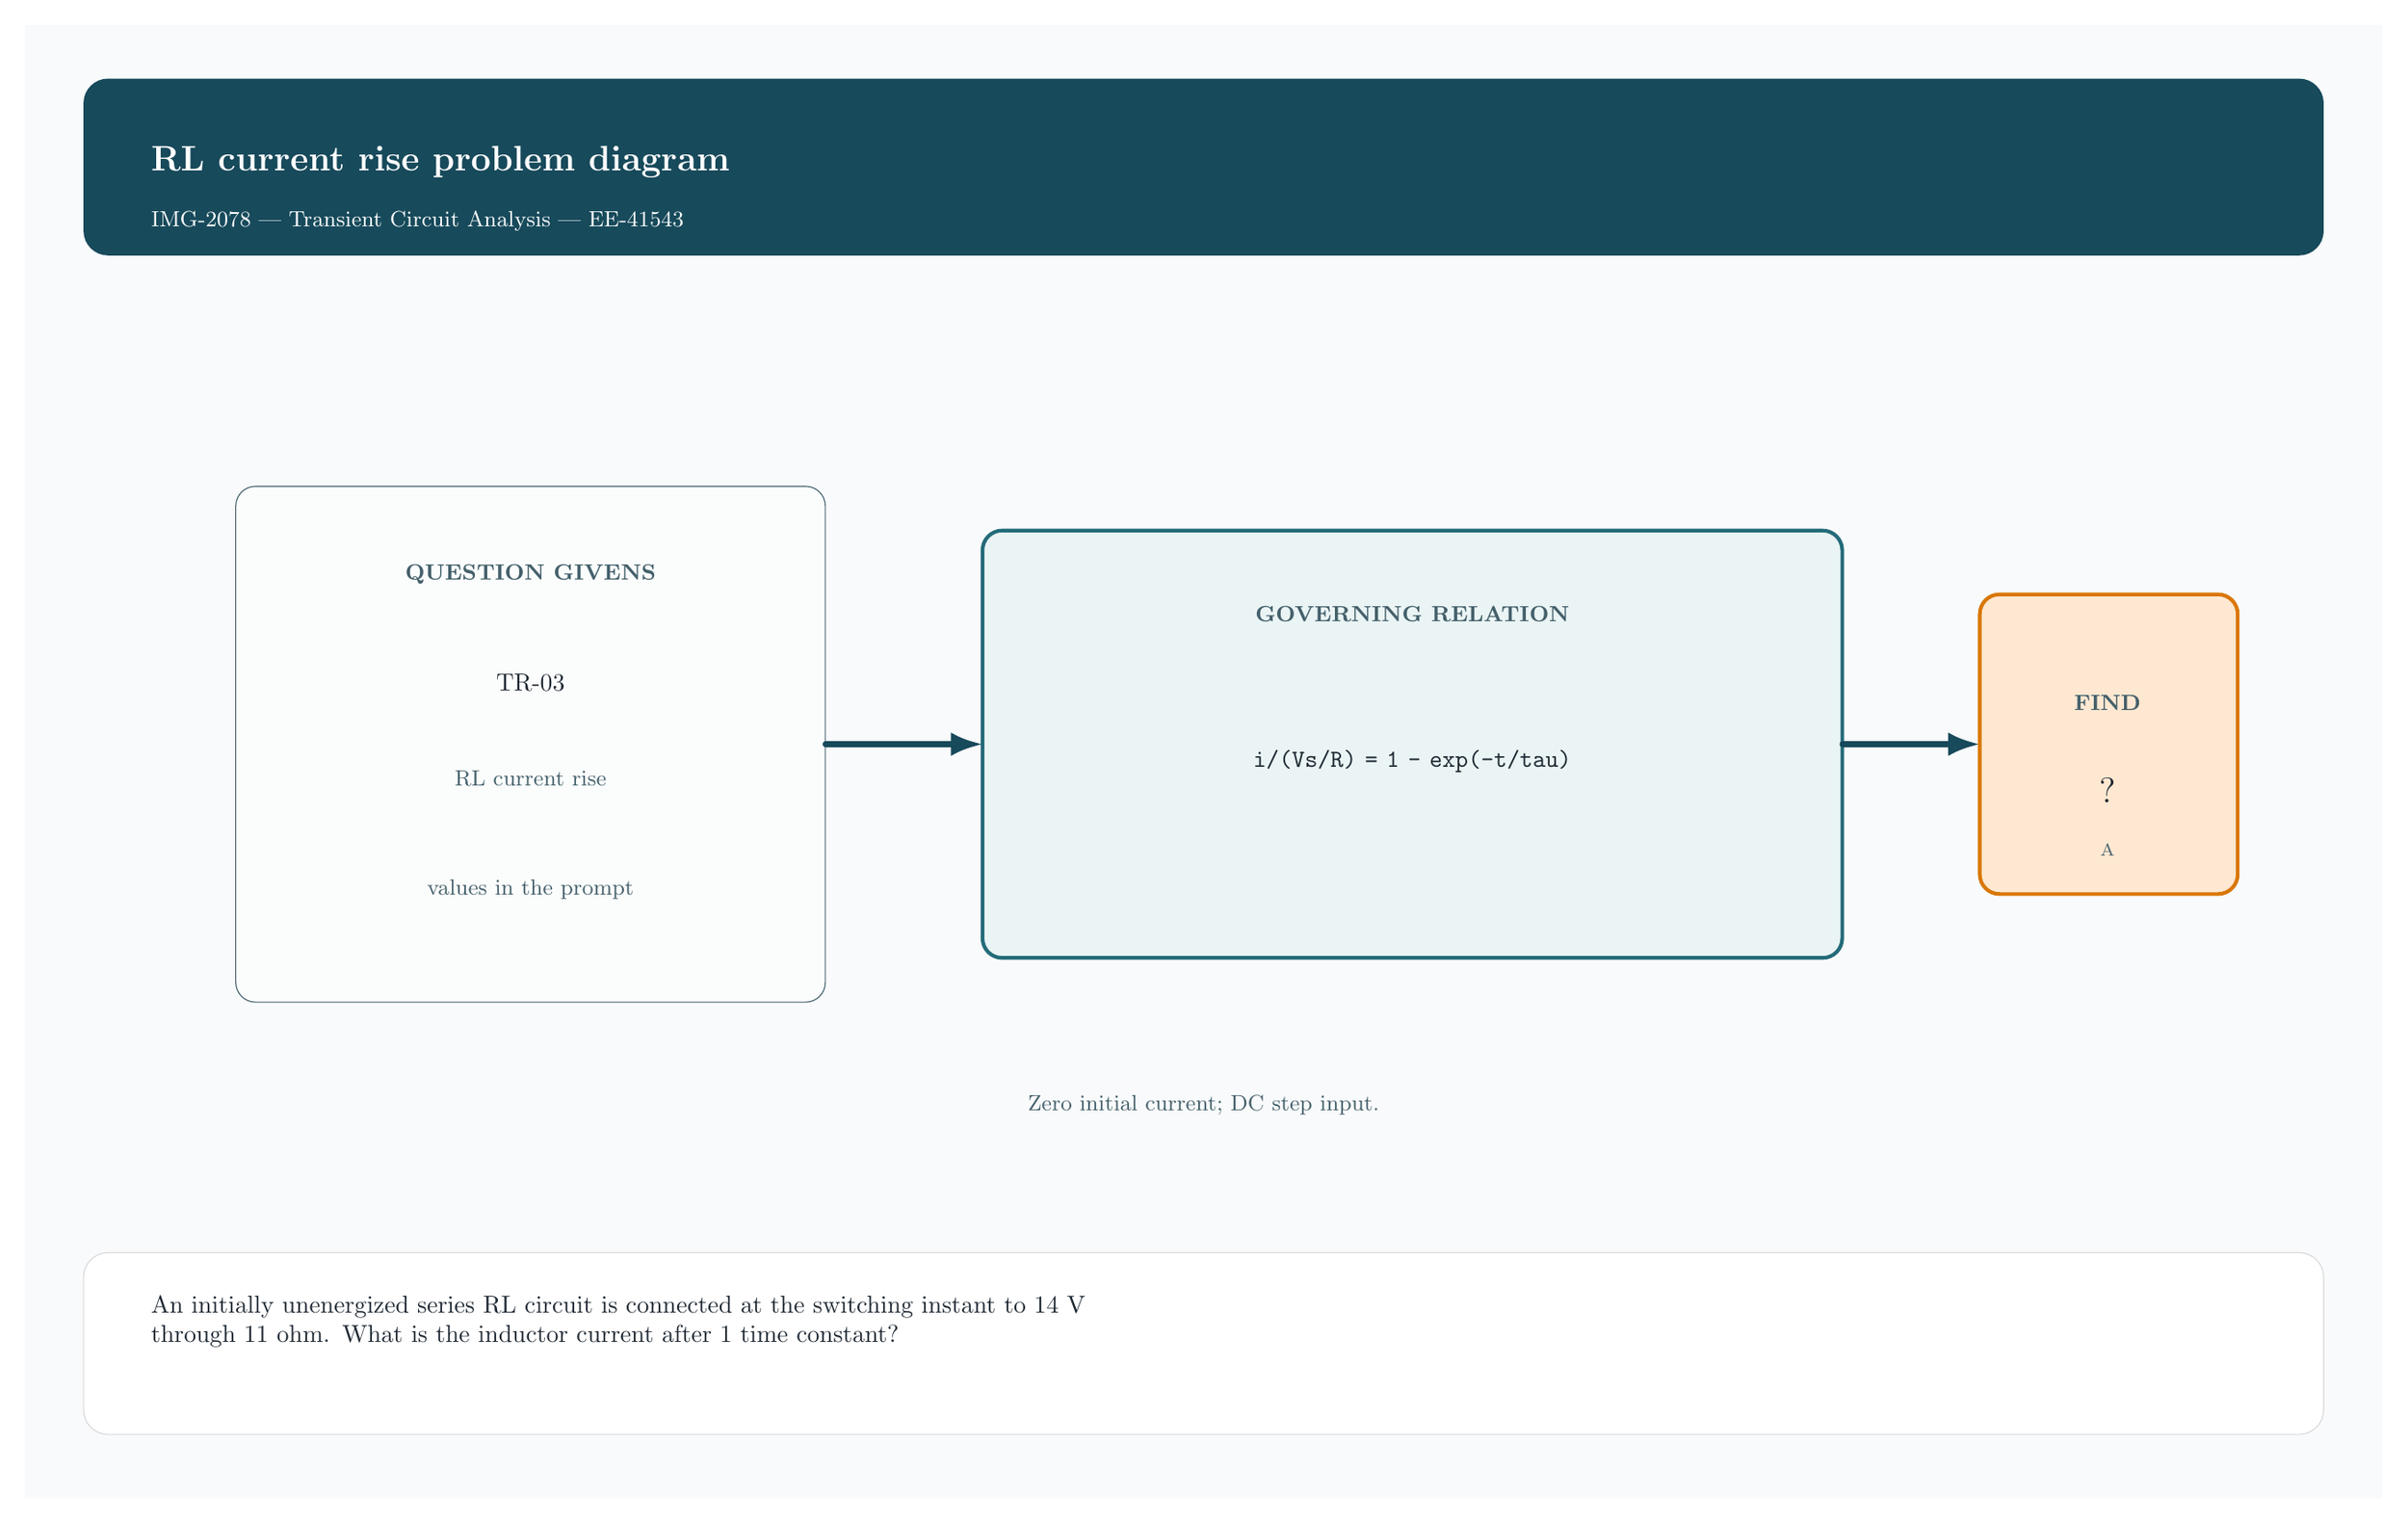
\begin{tikzpicture}[x=1pt,y=-1pt,>=Latex,line cap=round,line join=round]
\path[fill=zyloPaper] (0,0) rectangle (960,600);
\path[fill=zyloTeal,rounded corners=10pt] (24,22) rectangle (936,94);
\node[anchor=west,text=white,font=\bfseries\Large] at (48,56) {RL current rise problem diagram};
\node[anchor=west,text=white!82,font=\small] at (48,80) {IMG-2078 | Transient Circuit Analysis | EE-41543};
\tikzset{wire/.style={draw=zyloTeal,line width=2.2pt},thinwire/.style={draw=zyloLine,line width=1.35pt},accent/.style={draw=zyloOrange,line width=2.2pt},box/.style={draw=zyloTealTwo,fill=zyloSoft,line width=1.5pt,rounded corners=8pt}}
\path[draw=zyloLine,fill=white!80!zyloSoft,rounded corners=8pt] (86,188) rectangle (326,398);
\node[font=\small\bfseries,text=zyloLine] at (206,224) {QUESTION GIVENS};
\node[text=zyloInk] at (206,268) {TR-03};
\node[font=\small,text=zyloLine,text width=205pt,align=center] at (206,307) {RL current rise};
\node[font=\small,text=zyloLine] at (206,352) {values in the prompt};
\draw[wire,->] (326,293) -- (390,293);
\node[box,minimum width=350pt,minimum height=174pt] at (565,293) {};
\node[font=\small\bfseries,text=zyloLine] at (565,240) {GOVERNING RELATION};
\node[font=\ttfamily,text=zyloInk,text width=310pt,align=center] at (565,300) {i/(Vs/R) = 1 - exp(-t/tau)};
\draw[wire,->] (740,293) -- (796,293);
\path[draw=zyloOrange,fill=orange!18,rounded corners=8pt,line width=1.5pt] (796,232) rectangle (901,354);
\node[font=\small\bfseries,text=zyloLine] at (848,276) {FIND};
\node[font=\Large,text=zyloInk] at (848,312) {?};
\node[font=\scriptsize,text=zyloLine] at (848,336) {A};
\node[font=\small,text=zyloLine,text width=820pt,align=center] at (480,440) {Zero initial current; DC step input.};
\path[draw=black!15,fill=white,rounded corners=10pt] (24,500) rectangle (936,574);
\node[anchor=west,text width=860pt,align=left,text=zyloInk,font=\normalsize] at (48,528) {An initially unenergized series RL circuit is connected at the switching instant to 14 V\\through 11 ohm. What is the inductor current after 1 time constant?};
\end{tikzpicture}
\end{document}
